\documentclass{article}

\usepackage[utf8]{inputenc}
\usepackage[T1]{fontenc}
\usepackage[english]{babel}

\usepackage{amsfonts}
\usepackage{amsmath}
\usepackage{amssymb}
\usepackage{authblk}
\usepackage{csquotes}
\usepackage[pdf]{graphviz}
\usepackage{mathtools}
\usepackage{pdfpages}
\usepackage[detect-weight=true]{siunitx}
\usepackage{stmaryrd}
\usepackage{todonotes}

\usepackage[url=false]{biblatex}
\addbibresource{minimum.bib}

\newcommand{\email}[1]{\href{mailto:#1}{#1}}

% Multi-letter identifier
\newcommand{\mli}[1]{\mathit{#1}}

\DeclareMathOperator{\re}{\mathbb{R}}
\DeclareMathOperator{\nat}{\mathbb{N}}
\DeclareMathOperator{\logit}{logit}
\DeclareMathOperator{\sigmoid}{sigmoid}
\DeclareMathOperator*{\argmin}{argmin}
\DeclareMathOperator{\argsort}{argsort}
\newcommand{\inv}[1]{#1^{-1}}
\DeclarePairedDelimiter{\card}{\lvert}{\rvert}
\DeclarePairedDelimiter{\SquareBracket}{[}{]}
\DeclarePairedDelimiter{\Parentheses}{(}{)}
\DeclarePairedDelimiter{\ceil}{\lceil}{\rceil}
\newcommand{\DotProd}[2]{\left<#1,#2\right>}
\newcommand{\Better}[3]{#1 \prec_{#3} #2}
\newcommand{\Prob}[1]{\mathrm{Prob}(#1)}

\DeclareMathOperator{\symbols}{\Sigma}
\newcommand{\Problems}[1]{\mathcal{P}_{#1}}
\DeclareMathOperator{\cnf}{\Problems{\mathrm{CNF}}}
\DeclareMathOperator{\ProblemsTptp}{\Problems{0}}
\DeclareMathOperator{\ProblemsTrain}{\Problems{\mathrm{train}}}
\DeclareMathOperator{\ProblemsTrainEx}{\ProblemsTrain'}
\DeclareMathOperator{\ProblemsVal}{\Problems{\mathrm{val}}}
\DeclareMathOperator{\ProblemsValEx}{\ProblemsVal'}
\newcommand{\signature}[1]{\Sigma_#1}

% Precedences
\newcommand{\PrecBetter}{\pi}
\newcommand{\PrecWorse}{\rho}

\newcommand{\Vampire}{Vampire}

\newcommand{\loss}{\ell}
% Inspiration: The Elements of Statistical Learning, p. 120

\newcommand{\rewrite}[1]{\overset{#1}{\longrightarrow}}

\newcommand{\Conj}{C}
\newcommand{\NegConj}{\mli{NC}}
\newcommand{\AxiomS}{A_s}
\newcommand{\AxiomZ}{A_0}
\newcommand{\RulePS}{R_{+s}}
\newcommand{\RuleSP}{R_{s+}}
\newcommand{\RuleN}[1]{R_{#1}}



\begin{document}

\maketitle

\begin{abstract}
The state-of-the-art superposition-based theorem provers for \acrlong{fol} rely on simplification orderings on terms to constrain the applicability of inference rules,
which in turn shapes the ensuing search space.
The popular Knuth-Bendix simplification ordering is parameterized by symbol precedence---a permutation of the predicate and function symbols of the input problem’s signature.
Thus, the choice of precedence has an indirect yet often substantial impact on the amount of work required to complete a proof search successfully.

This work describes and evaluates two approaches to the construction of a symbol precedence recommender.
Each of them uses machine learning to predict the best possible precedence.
Both recommenders are trained on observations of prover performance on a set of problems and random precedences.
The first approach uses a small set of simple human-engineered symbol features.
The second approach uses a \acrfull{gcn} to extract meaningful symbol embeddings from the graph structure of the input problem.
When coupled with the theorem prover Vampire and evaluated on the \acrshort{tptp} problem library, the \acrshort{gcn}-based recommender is found to outperform a state-of-the-art heuristic by more than \SI{4}{\percent} on unseen problems.

\end{abstract}

\section{Introduction}

Automated theorem proving is a classical field of \acrlong{ai} \cite{Russell2010}.
Given a sentence written in a formal system such as the \acrlong{fol},
an \gls{atp} searches for a formal proof of the sentence.
In the last decades, a number of efficient \glspl{atp} have been implemented,
together with many search heuristics necessary to navigate the search space.
These systems are today increasingly used as black-box reasoners in disciplines
such as mathematics \cite{DBLP:conf/birthday/KinyonVV13},
software and hardware verification \cite{Ahrendt2016,Hunt2017},
common-sense reasoning \cite{Pease2010},
and legal reasoning \cite{Passmore2017}.

\Gls{fol} strikes an attractive balance between expressive strength and efficient automated reasoning.
Theorem proving based on the saturation paradigm \cite{DBLP:books/el/RV01/BachmairG01}
represents the state-of-the-art method for automatically proving conjectures in \gls{fol}.
This technology combines several highly nontrivial techniques,
including the use of refutationally complete logical calculi \cite{DBLP:books/el/RV01/NieuwenhuisR01},
powerful redundancy criteria \cite{DBLP:books/el/RV01/BachmairG01},
and advanced indexing \cite{Voronkov1995}.

Despite the ongoing improvements of \gls{atp} systems, with small exceptions,
\glspl{atp} are still significantly weaker than trained mathematicians in finding proofs in most research domains.
At the same time, the area of \gls{ml} and, in particular, the use of deep artificial neural networks has recently seen a number of advances which came hand in hand with several breakthroughs in various application domains.
Examples include \acrlong{cv} \cite{CHAI2021100134},
\acrlong{nlp} \cite{8949185}, and
playing computer games \cite{shao2019survey}.
These recent impressive advances in machine learning manifested in a number of domains suggest to apply such techniques also in the \gls{atp} field.

\section{Related work}

Thus far, the most successful applications of \gls{ml} in automated theorem proving have been in a high-level external setting of selecting a small number of relevant facts (axioms, definitions, theorems) for proving new conjectures over large formal libraries \cite{DBLP:journals/jar/AlamaHKTU14,DBLP:journals/jar/BlanchetteGKKU16,DBLP:conf/cpp/GauthierK15}.
This has become known as the premise selection task.

More recently, \gls{ml} has also started to be used to guide the internal search of the \gls{atp} systems.
This means providing advice when the \gls{atp} is choosing among many possible inference steps of its non-deterministic proof calculus.
This is more challenging, because the trained machine learner is typically called thousands of times during the proof search and thus needs to be both fast and efficiently integrated with the core \gls{atp} system.

In the simpler connection tableau systems such as leanCoP \cite{10.1007/978-3-540-71070-7_23}, supervised learning has been used to choose the next tableau extension step \cite{DBLP:journals/jar/FarberKU21} and first experiments with Monte-Carlo guided proof search and reinforcement learning have been done, recently outperforming the unguided systems by \SI{40}{\percent} on standard benchmarks \cite{DBLP:conf/nips/KaliszykUMO18}.
In saturation-style provers, this has been done by feedback loops for strategy invention \cite{DBLP:journals/aicom/JakubuvU18,DBLP:conf/gcai/SchaferS15} and by using supervised learning \cite{DBLP:conf/cade/JakubuvCOP0U20,DBLP:conf/lpar/LoosISK17} to select the next given clause \cite{McCune2003}.

\section{Objectives}

The main objective of my research is an investigation of novel ways of increasing the performance of state-of-the-art saturation-based \glspl{atp} by using \gls{ml}.
The \gls{atp} Vampire \cite{DBLP:conf/cav/KovacsV13} serves as the primary target system of interest
mainly due to its relative strength
as testified by the annual \gls{casc} \cite{Sut16}.

\subsection{Symbol precedence construction}

Vampire uses the superposition calculus \cite{DBLP:journals/logcom/BachmairG94,DBLP:books/el/RV01/NieuwenhuisR01} as its inference system.
The superposition calculus is restricted by a \gls{sot},
which is usually specified by a symbol precedence---a permutation of the input problem signature.

In the first phase of this research project, I experimented with generating good symbol precedences by \gls{ml}.
These experiments have been described in detail in two publications:
\begin{enumerate}
\item Learning Precedences from Simple Symbol Features \cite{DBLP:conf/cade/Bartek020}:
A precedence recommender based on simple syntactic symbol features published at \gls{paar-2020}
\item Neural Precedence Recommender \cite{DBLP:conf/cade/Bartek021}:
A precedence recommender based on a \gls{gcn} published at \gls{cade-28}
\end{enumerate}
Copies of these two publications form the last part of this document.

\subsection{Strategy schedule construction}

A typical modern \gls{atp} such as Vampire employs a large number of parameterized proof search heuristics.
The combination of these parameters gives rise to a large number of possible proving strategies.
It is usually very hard to predict the behavior of a particular strategy on a given input problem.
At the same time, a great improvement in performance can be achieved by using a combination of multiple proving strategies assembled into portfolios, executed either sequentially (as a strategy schedule) \cite{DBLP:conf/cade/Tammet98} or in parallel.

In the second phase of this research project, I will experiment with the invention of strategy schedules for the \gls{atp} Vampire.
The existing approaches to strategy schedule invention first discover a set of strategies and then compose a schedule of these strategies
\cite{DBLP:journals/jar/KuhlweinU15,DBLP:journals/aicom/JakubuvU18,DBLP:conf/mkm/HoldenK21}.
My aim is to integrate the strategy and schedule optimization more tightly,
evaluating the partially constructed schedule repeatedly
to steer the search towards strategies that complement the current portfolio.

\clearpage
\printbibliography

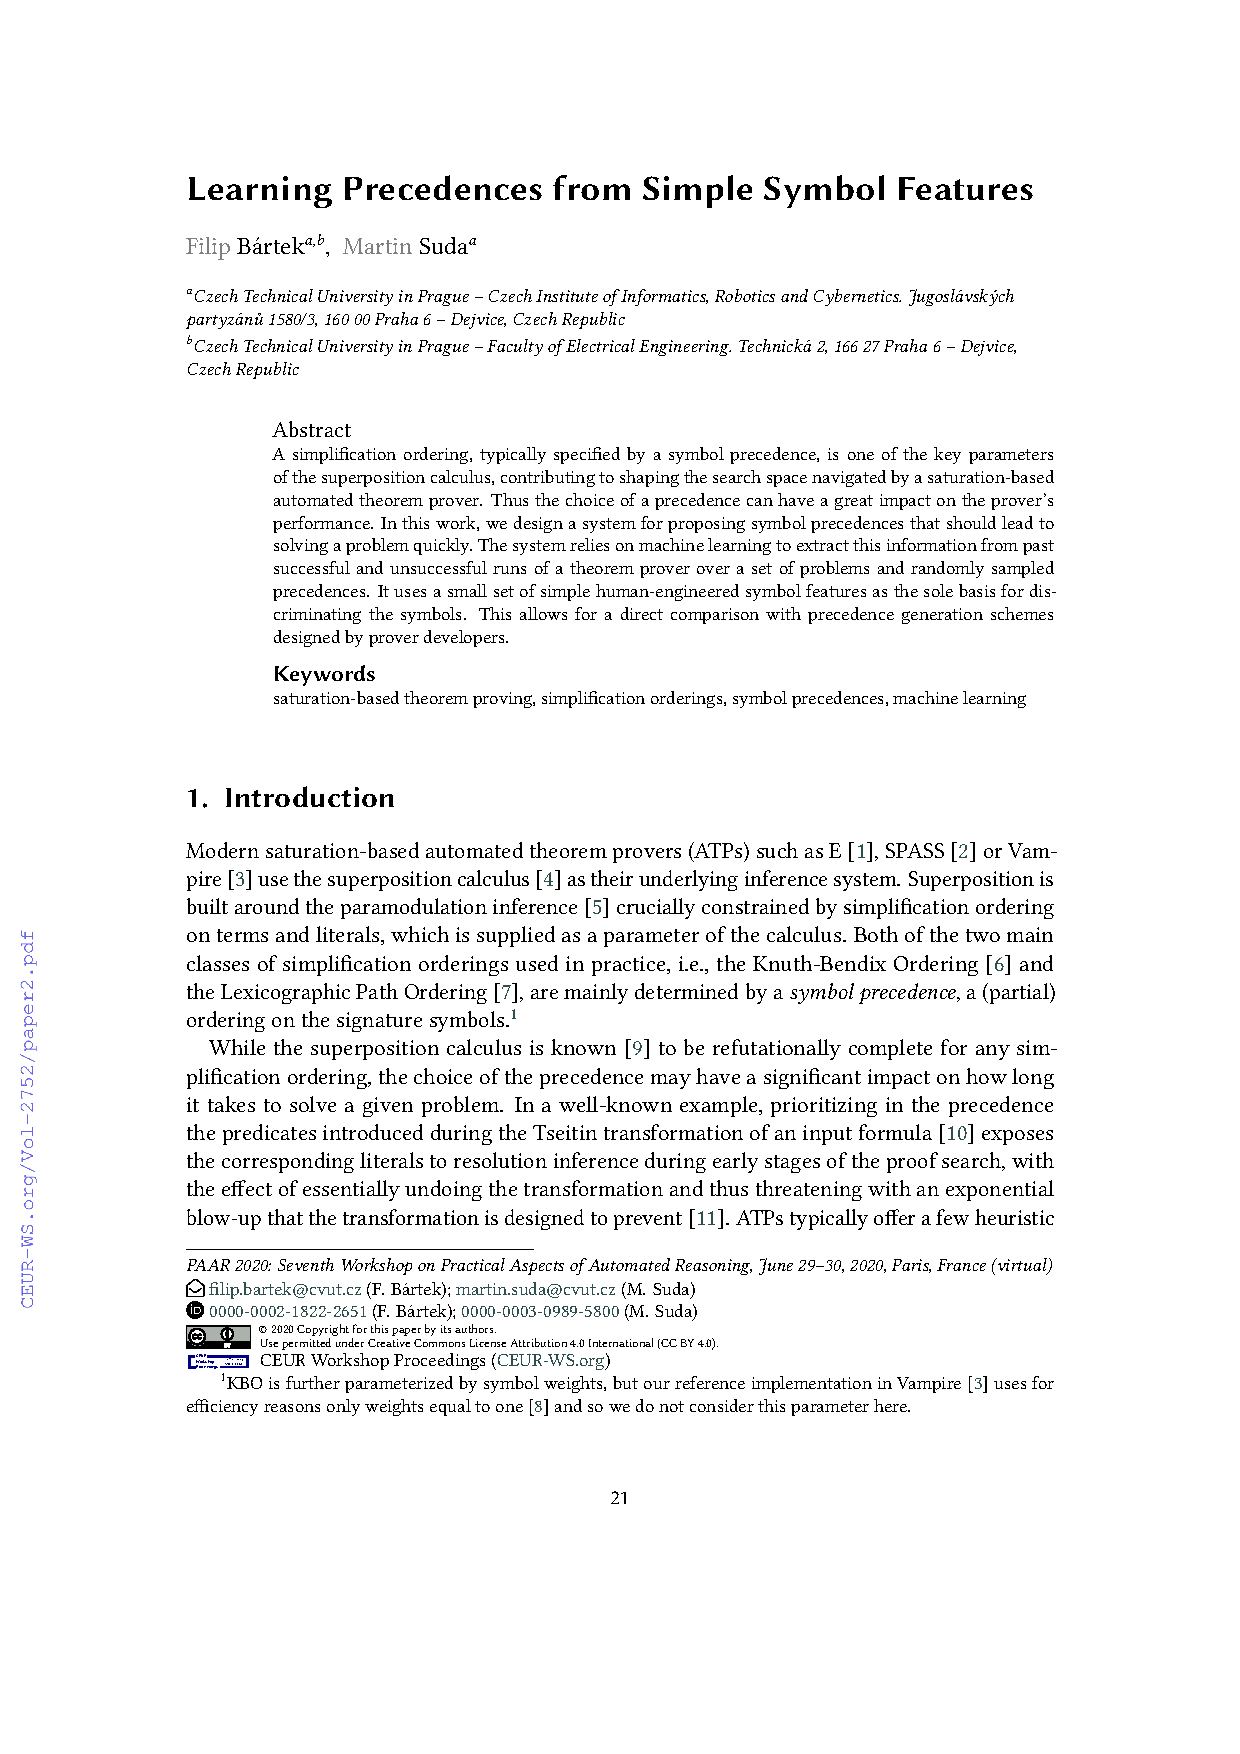
\includepdf[pages=-]{papers/2020-paar.pdf}
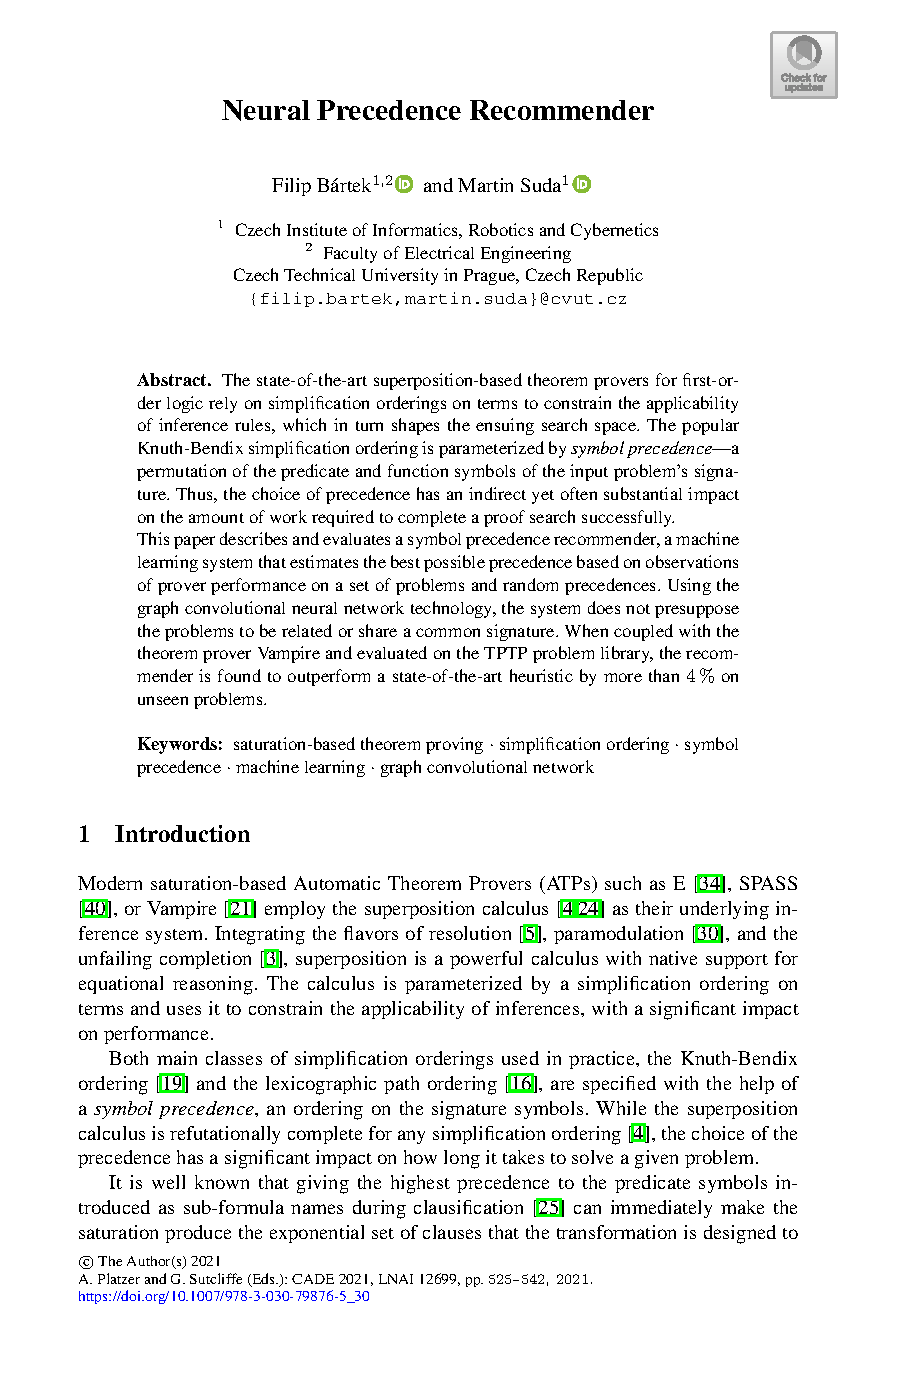
\includepdf[pages=-]{papers/2021-cade.pdf}

\end{document}
